% !TeX spellcheck = da_DK
\subsection{ADC}\label{ADC_afsnit}
\subsubsection{Teori og design}
I dette projekt anvendes en ADC af typen NI USB-6009 til at konvertere det analoge signal til digital. %Signalet skal konverteres, for at kunne sendes ind i den digitale del af systemet, så plejepersonalet kan aflæse og behandle målingerne. 
Med denne ADC kan der samples med $13$ bits single-ended. ADC'en kan dermed inddeles i $2^{13} = 8192$ niveauer, jævnfør afsnit \ref{ADCafsnit}, side \pageref{ADCafsnit}. Den maksimale samplingsrate er på $48$kS/s\fxnote{NTK: Kilo samples pr. sekund}, hvormed det er muligt at sample med minimum det tidobbbelte af båndbredden. Arbejdsområdet for ADC'en ligger på $\pm10$V og har en typisk præcision på $14.7$mV ved $25^{\circ}$C. \cite{Instruments2014} LSB udregnes vha. \eqref{ligningLSB}, side \pageref{ligningLSB}. %er det muligt at udregne LSB vha. ligningen i afsnit \ref{ADCafsnit} på side \pageref{ADCafsnit}. Udregningen ser således ud: \\
%\begin{equation}
%	LSB = \frac{FSR}{2^{n}} 
%\end{equation}  
%FSR er arbejdsområdet, dvs. $10Vpp$, som indsættes i formlen som $20V$, imens n er antallet af bits, der kan samples med, dvs. $13$.
Værdierne indsættes i formlen: \\
\begin{align}
	LSB = \frac{20V}{2^{13}}
	LSB = 0.00244V = 2.44\text{mV}
\end{align}
Det opsamlede signal forvrænges, og vil dermed ikke være repræsentativt, hvis der opsamles værdier på under $2.44mV$.\\
\subsubsection{Simulering}
Jævnfør kravspecifikationerne i afsnit \ref{ADC_kravspecifikation}, side \pageref{ADC_kravspecifikation} skal der testes for, hvorvidt ADC'en kan modtage og konvertere et inputsignal på $\pm4$V samt sample $250$ gange i sekundet. \\
Der kan ikke laves en simulering af ADC'en i programmet LTspice, da der ikke kan dannes et analogt signal i LTspice, som skal konverteres.
 
\subsubsection{Implementering og test}
%ADC'en skal implementeres og tilkobles efter lavpasfiltret, som det kan ses på \figref{kravblok} på side \pageref{kravblok}. \\
Der benyttes en funktionsgenerator til at undersøge, hvorvidt den valgt ADC overholder kravene, jævnfør afsnit \ref{ADC_kravspecifikation}, side \pageref{ADC_kravspecifikation}. Funktionsgeneratoren skal sende fem forskellige input til ADC'en;
\begin{enumerate}
	\item Et sinussignal med en frekvens på $100$Hz og den højeste forventede amplitude, dvs. $0.3313 \cdot 9.1 = 3.0148$V.
	\item Et sinussignal med en frekvens på $100$Hz og den laveste forventede amplitude, dvs. -$0.3233 \cdot 9.1 = $-$2.9420$V.
	\item Et sinussignal med en frekvens på $25$Hz og en amplitude på $4$V, da der ses i \tableref{Tab:faktor3_test}, at operationsforstærkerne går i mætning ved ca. $4$V, når de forsynes med $5.5$V. 
	\item Et sinussignal med en frekvens svarende til pasbåndsfrekvensen i lavpasfiltret, dvs. $25$Hz, og den højeste forventede amplitude, dvs. $0.3313 \cdot 9.1 = 3.0148$V.
	\item Et sinussignal med en frekvens svarende til pasbåndsfrekvensen i lavpasfiltret, dvs. $25$Hz, og den laveste forventede amplitude, dvs. -$0.3233 \cdot 9.1 = $-$2.9420$V.
\end{enumerate}
\noindent Der samples med $500$Hz, selvom $250$Hz havde været nok, da signalets båndbredde er $25$Hz, men ScopeLogger kan enten sample med $200$ eller $500$. På \figref{fig:ADC_Test} ses resultatet af målingerne.

\begin{figure}[H]
	\centering
	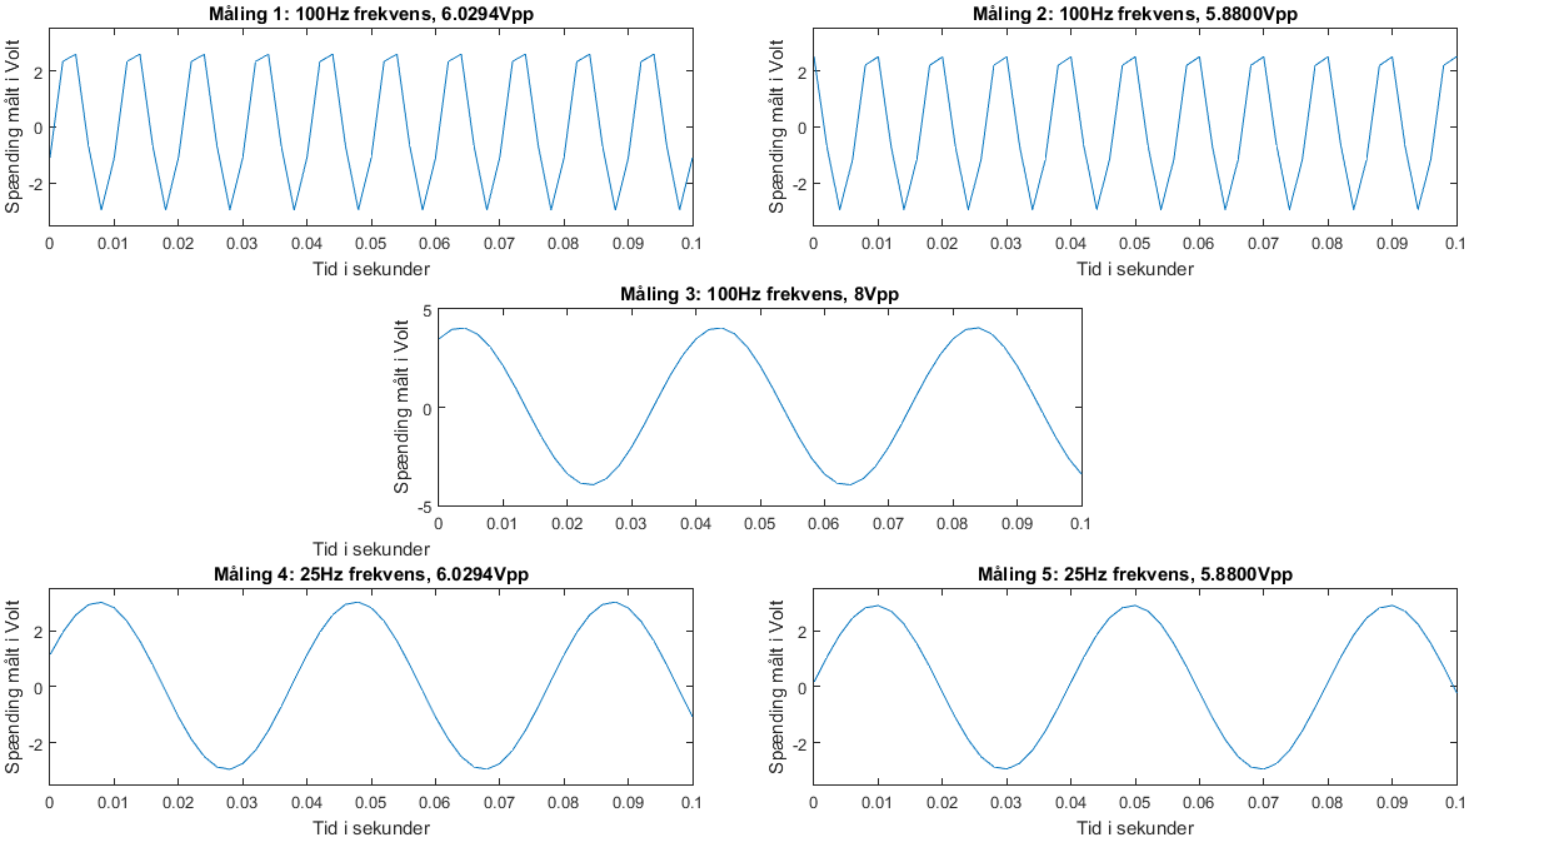
\includegraphics[scale=0.45]{figures/cProblemloesning/ADC_Test2_matlab.PNG}
	\caption{På figuren ses resultatet af de fem målinger plottet i MATLAB. Overskiften til hver graf beskriver amplituden og frekvensen for signalet i hver måling. Der ses, at x-aksen for alle plots er afgrænset til 0.1 sekund.}
	\label{fig:ADC_Test}
\end{figure}

\noindent Dataen optaget med ADC'en, som er plottet i \figref{fig:ADC_Test}, bliver efterfølgende bearbejdet i MATLAB. Derudover bliver et oscilloskop tilkoblet outputtet fra funktionsgeneratoren. Resultatet herfra betragtes som det faktiske output fra funktionsgeneratoren, hvilket indgår i beregningen af afvigelsen i ADC'ens sampling. Resultaterne ses i \tableref{Tab:ADC_resultat}:

\begin{table}[H]
	\centering
	\begin{tabular}{|l|l|l|l|l|l|}
		\hline
		\textit{Måling nr} & \textit{\begin{tabular}[c]{@{}l@{}}Indstillet\\ frekvens\end{tabular}} & \textit{\begin{tabular}[c]{@{}l@{}}Indstillet\\ amplitude\end{tabular}} & \textit{\begin{tabular}[c]{@{}l@{}}Målte amplitude\\ på oscilloscop\end{tabular}} & \textit{\begin{tabular}[c]{@{}l@{}}Målte amplitude\\ via ADC\end{tabular}} & \textit{Afvigelse} \\ \hline
		\textit{$1$}         & $100$Hz     & $3.0147$V    & $3.0800$V      & $2.5989$V       & $15.62$\%          \\ \hline
		\textit{$2$}         & $100$Hz     & $2.9400$V    & $2.9200$V      & $2.5284$V       & $13.32$\%          \\ \hline
		\textit{$3$}         & $25$Hz      & $4$V         & $4.0400$V      & $4.0442$V       & $0.10$\%           \\ \hline
		\textit{$4$}         & $25$Hz      & $3.0147$V    & $3.0800$V      & $3.0689$V       & $0.36$\%           \\ \hline
		\textit{$5$}         & $25$Hz      & $2.9400$V    & $2.9200$V      & $2.9207$V       & $0.02$\%           \\ \hline
	\end{tabular}
	\caption{I tabellen ses resultaterne af det målte signal med hhv. et oscilloskop og ADC'en. Oscilloskopets måling vurderes som det faktiske output og derved kan afvigelserne beregnes.}
	\label{Tab:ADC_resultat}
\end{table}
\noindent Det kan ses på \figref{fig:ADC_Test}, at det samplede signal i måling $1$ og $2$ er mere kantet end signalerne i måling $3$-$5$. Årsagen til dette er, at der samples med $500$Hz, mens signalets frekvens er $100$Hz. Dette gør, at ADC'en sampler med $5$ gange pr. periode og derved bliver signalet kantet. Derfor giver ADC'ens værdi for amplituden en afvigelse på hhv. $15.62\%$ og $13.32\%$, da samplingsfrekvensen ikke passer til signalets frekvens. Det vurderes dermed, at det er samplingsfrekvensen, som er den primære årsag til de høje afvigelser.\\
I måling $3$-$5$ er sinussignalets frekvens nedsat, hvilket gør, at signalet bliver mere regelmæssigt. Der samples med en samplingsfrekvens, der er $20$ gange større end frekvensen, og der opsamles derved tilstrækkeligt med datapunkter. Derfor er procentafvigelserne fra måling $3$-$5$ mere repræsentative for ADC'ens afvigelse. Afvigelserne kan også skyldes tolerancer i oscilloskopet. Der vurderes derfor, at ADC'en viser det forventede. ADC'en opfylder blokkens tolerancer, hvorfor den accepteres.